%% To change chapter header dynamically from french to english, use
%%\entetedynamique
\setcounter{corA}{0} % Pour recommancer à compter les def,
                     % theo, etc. à partir de 1
 % Pour écrire un article en français
\francais
 % Pour écrire un article en anglais
%%\anglais
%% NOTE: La plupart des macros ont un nom en anglais.
%% P.ex. \adresse et \address fonctionnent et sont équivalents.
%% \revue=\journal
%% \auteur=\author
%% \titre=\title

 % Nom de la revue de publication
\revue{Une revue}
\article{Titre de l'article}

 % Contribution(s) peronnelle(s) à l'article et rôle joué par tous les coauteurs
 %
 % Nécessaire seulement lorsque vous n'êtes pas seul·e auteur·e.
 % Les contributions peuvent apparaître ailleur dans la thèse.
 % Si \contributions est laissé vide (p.ex. si vous effacez
 % celui ci-bas), aucune contributions ne seront générées sur
 % la page titre de l'article.
 %
 % REMARQUE : L'exemple est sous forme d'\itemize,
 % mais toutes les constructions \LaTeX\ sont permises.
 % La commande peut aussi contenir un simple petit texte.
 %
 % La commande admet une option [<entête>]
\contributions%[Mes contributions et le rôle des coauteurs]
{
    \begin{itemize}
        \item Calcul de telle chose;
        \item Vérification de telle équation;
        \item Idée pour telle définition;
        \item Démonstration de tel théorème.
    \end{itemize}

    Le coauteur1 a suggéré telle chose.

    Le coauteur2 a fait telle calcul.\\[1cm]
}
%% Les contributions apparaîtrons après
%% \maketitle. Selon les goûts, il est
%% possible de mettre les contributions
%% avant, simplement en les écrivant
%% directement ici. Par exemple :
 % \section*{Contributions de <mon nom> et rôle joué par les coauteurs}
 % J'ai contribué en...
 %
 % Le rôle des coauteurs a été de...
 % \cleardoublepage

%%% INFORMATIONS POUR LA PAGE TITRE
 % Premier auteur·e et adresse
\auteur{Hima Ginère}
\adresse{1252i rue complexe\\ Université du plan complexe}
 % Deuxième auteur·e et adresse (si différente de la première)
%%\auteur{Hana Lietick}
%%\adresse{4242 rue imaginaire\\ Universität von der gau\ss sche Zahlenebene}
%%
%% et ainsi de suite pour les autres auteurs

\maketitle

\begin{resume}{Mots clés}
  Le résumé en français.
\end{resume}

\begin{abstract}{Key words}
  The english abstract.
\end{abstract}

\section{Introduction}
%%
%% Le reste de l'article...
%%

% Options for packages loaded elsewhere
\PassOptionsToPackage{unicode}{hyperref}
\PassOptionsToPackage{hyphens}{url}
%
\documentclass[
]{article}
\usepackage{amsmath,amssymb}
\usepackage{lmodern}
\usepackage{ifxetex,ifluatex}
\ifnum 0\ifxetex 1\fi\ifluatex 1\fi=0 % if pdftex
  \usepackage[T1]{fontenc}
  \usepackage[utf8]{inputenc}
  \usepackage{textcomp} % provide euro and other symbols
\else % if luatex or xetex
  \usepackage{unicode-math}
  \defaultfontfeatures{Scale=MatchLowercase}
  \defaultfontfeatures[\rmfamily]{Ligatures=TeX,Scale=1}
\fi
% Use upquote if available, for straight quotes in verbatim environments
\IfFileExists{upquote.sty}{\usepackage{upquote}}{}
\IfFileExists{microtype.sty}{% use microtype if available
  \usepackage[]{microtype}
  \UseMicrotypeSet[protrusion]{basicmath} % disable protrusion for tt fonts
}{}
\makeatletter
\@ifundefined{KOMAClassName}{% if non-KOMA class
  \IfFileExists{parskip.sty}{%
    \usepackage{parskip}
  }{% else
    \setlength{\parindent}{0pt}
    \setlength{\parskip}{6pt plus 2pt minus 1pt}}
}{% if KOMA class
  \KOMAoptions{parskip=half}}
\makeatother
\usepackage{xcolor}
\IfFileExists{xurl.sty}{\usepackage{xurl}}{} % add URL line breaks if available
\IfFileExists{bookmark.sty}{\usepackage{bookmark}}{\usepackage{hyperref}}
\hypersetup{
  pdftitle={Test},
  pdfauthor={Author Name},
  hidelinks,
  pdfcreator={LaTeX via pandoc}}
\urlstyle{same} % disable monospaced font for URLs
\usepackage{graphicx}
\makeatletter
\def\maxwidth{\ifdim\Gin@nat@width>\linewidth\linewidth\else\Gin@nat@width\fi}
\def\maxheight{\ifdim\Gin@nat@height>\textheight\textheight\else\Gin@nat@height\fi}
\makeatother
% Scale images if necessary, so that they will not overflow the page
% margins by default, and it is still possible to overwrite the defaults
% using explicit options in \includegraphics[width, height, ...]{}
\setkeys{Gin}{width=\maxwidth,height=\maxheight,keepaspectratio}
% Set default figure placement to htbp
\makeatletter
\def\fps@figure{htbp}
\makeatother
\setlength{\emergencystretch}{3em} % prevent overfull lines
\providecommand{\tightlist}{%
  \setlength{\itemsep}{0pt}\setlength{\parskip}{0pt}}
\setcounter{secnumdepth}{-\maxdimen} % remove section numbering
\usepackage[]{minted}
\setminted{breaklines=true}
\ifluatex
  \usepackage{selnolig}  % disable illegal ligatures
\fi

\title{Test}
\author{Author Name}
\date{}

\begin{document}
\maketitle

\hypertarget{summary}{%
\section{Summary}\label{summary}}

Predicting where species should be found in space is a common question
in ecology and biogeography. Species distribution models (SDMs), for
instance, aim to predict where environmental conditions are suitable for
a given species, often on continuous geographic scales. Such analyses
require the use of geo-referenced data on species distributions coupled
with climate or land cover information, hence a tight integration
between environmental data, species occurrence data, and spatial
coordinates. Thus, it requires an efficient way to access these
different data types within the same software, as well as a flexible
framework on which to build various analysis workflows. Here we present
\mintinline[]{text}{SimpleSDMLayers.jl} and
\mintinline[]{text}{GBIF.jl}, two packages in the \emph{Julia} language
implementing a simple framework and type-system on which to build SDM
analyses, as well as providing access to popular data sources for
species occurrences and environmental conditions.

\hypertarget{statement-of-need}{%
\section{Statement of need}\label{statement-of-need}}

Species distribution modeling (SDM) is an increasingly growing field in
ecology and biogeography, with many applications in biodiversity
assessment, management, and conservation {[}@Araujo2019StaDis{]}. Most
SDM models aim at predicting a species distribution in space based on
environmental data and information on where the species was previously
seen. Hence, SDM studies require a tight and efficient integration
between geo-referenced environmental and species occurrence data.
However, such data are complex to handle and often require different
software: climate and land use data are stored as layers in raster
files, then visualized and manipulated in specialized GIS (geographic
information systems) software, while occurrence data are stored in
tables and spreadsheets, then manipulated in data analysis and
statistics-oriented tools or programming languages. Therefore, there is
a need for efficient tools to manipulate bioclimatic data, specifically
oriented towards species distribution modeling.

In recent years, \emph{R} {[}@RCoreTeam2020RLan{]} has become the most
widely used programming language in ecology, especially in spatial
ecology studies {[}@Lai2019EvaPop{]}. Hence, many efficient packages and
tools for species distribution modeling have been developed in \emph{R}.
For instance, the package \mintinline[]{text}{raster}
{[}@Hijmans2020RasGeo{]} can be used to manipulate raster format data
(for example climatic or land use data), \mintinline[]{text}{dismo}
{[}@Hijmans2017DisSpe{]} implements many SDM models and provides access
to common climatic data sources, and \mintinline[]{text}{rgbif}
{[}@Chamberlain2020RgbInt{]} provides access to the GBIF database, a
common source of species occurrence data in SDM studies. In comparison,
few specific SDM resources currently exist for the \emph{Julia} language
{[}@Bezanson2017JulFre{]}, although SDM models could benefit from its
speed, efficiency and ease of writing (removing the need to rewrite
functions in other languages for higher performance, as in \emph{R}).
There are currently packages such as
\href{https://github.com/JuliaGeo/GDAL.jl}{\mintinline[]{text}{GDAL.jl}}
and
\href{https://github.com/yeesian/ArchGDAL.jl}{\mintinline[]{text}{ArchGDAL.jl}}
to manipulate raster data; however, these are lower-level
implementations than what is typically used by most ecologists, and they
lack support for common layer manipulation. generalized linear models
(\href{https://github.com/JuliaStats/GLM.jl}{GLM.jl}), random forests
(\href{https://github.com/bensadeghi/DecisionTree.jl}{DecisionTrees.jl}),
neural networks (\href{https://github.com/FluxML/Flux.jl}{Flux.jl}), and
other commonly used models have excellent implementations in
\emph{Julia}, although not oriented towards species distribution
modeling and raster format data.

\mintinline[]{text}{SimpleSDMLayers.jl} is a package to facilitate
manipulation of geo-referenced raster data in \emph{Julia}, specifically
aimed at species distribution modeling. It is a higher-level
implementation, building on \mintinline[]{text}{ArchGDAL.jl}, that is
easier to use and provides support for common SDM operations (see
\emph{Feature Overview} section below). The package implements simple
type structures to manipulate the input and output data of SDM models,
and is meant to be a flexible framework on which to build more complex
analyses. While it does not implement SDM models in itself, we believe
the package is a step that will make \emph{Julia} more popular for
species distribution modeling, and lead to the development of more
complete implementations. \mintinline[]{text}{SimpleSDMLayers.jl} also
offers built-in access to some of the most common data sources in SDM
studies, such as the WorldClim 2.1 climatic data, which is the most
common source of climate data in SDM studies {[}@Booth2014BioFir{]}. The
package is also tightly integrated with \mintinline[]{text}{GBIF.jl},
which allows easy access to the GBIF database, a common data source for
species occurrences. Both \mintinline[]{text}{SimpleSDMLayers.jl} and
\mintinline[]{text}{GBIF.jl} are part of the \emph{EcoJulia}
organization, whose aim is to integrate a variety of packages for
ecological analyses in \emph{Julia}.

\hypertarget{basic-structure}{%
\section{Basic structure}\label{basic-structure}}

The core structure implemented in
\mintinline[]{text}{SimpleSDMLayers.jl} is the
\mintinline[]{text}{SimpleSDMLayer} type, with two variants,
\mintinline[]{text}{SimpleSDMPredictor} and
\mintinline[]{text}{SimpleSDMResponse}, depending if the layer is meant
to be mutable or not.

A \mintinline[]{text}{SimpleSDMLayer} element is made of a
\mintinline[]{text}{grid} field, which contains the raster data as a
simple \mintinline[]{text}{Array} (matrix) of any type, easily
manipulable. It also contains the fields \mintinline[]{text}{left},
\mintinline[]{text}{right}, \mintinline[]{text}{bottom}, and
\mintinline[]{text}{top}, representing the bounding coordinates of the
layer.

To illustrate this structure, the following code loads a layer of
WorldClim 2.1 climate data, which also shows how easily this can be done
in a single call. By default, this will return a layer with the values
for the whole world if no bounding coordinates are specified.

\begin{minted}[]{julia}
# Load package
using SimpleSDMLayers

# Get world temperature data
temperature = worldclim(1)
\end{minted}

\begin{minted}[]{text}
SimpleSDMLayers.SimpleSDMPredictor{Float32}(Union{Nothing, Float32}[-31.017
105f0 -31.62153f0 … -32.81253f0 -31.620333f0; -30.391916f0 -31.63478f0 … 
-32.81005f0 -30.995281f0; … ; nothing nothing … nothing nothing; nothing 
nothing … nothing nothing], -180.0, 180.0, -90.0, 90.0)
\end{minted}

The raster values can be displayed by calling the
\mintinline[]{text}{grid} field.

\begin{minted}[]{julia}
# Display data grid
temperature.grid
\end{minted}

\begin{minted}[]{text}
1080×2160 Array{Union{Nothing, Float32},2}:
 -31.0171    -31.6215    -31.6227    …  -32.8129    -32.8125    -31.6203
 -30.3919    -31.6348    -31.6341       -32.8092    -32.8101    -30.9953
 -33.4822    -34.1494    -34.1493       -35.4658    -35.4633    -34.1374
 -33.6104    -34.2875    -34.2865       -35.596     -35.5931    -34.2528
 -33.7199    -34.4041    -34.4014       -35.6932    -35.691     -34.3311
 -33.8224    -34.5184    -34.5162    …  -35.8037    -35.7996    -34.4165
 -31.6613    -32.3194    -32.3184       -33.5133    -33.5101    -32.2032
 -31.7635    -32.4307    -33.7036       -34.9522    -33.6282    -32.3038
 -33.7063    -36.0738    -39.2075       -40.6438    -37.3938    -34.3026
 -33.9768    -34.7016    -35.8662       -37.2408    -36.0364    -34.5988
                                                                
    nothing     nothing     nothing        nothing     nothing     nothing
    nothing     nothing     nothing        nothing     nothing     nothing
    nothing     nothing     nothing        nothing     nothing     nothing
    nothing     nothing     nothing        nothing     nothing     nothing
    nothing     nothing     nothing  …     nothing     nothing     nothing
    nothing     nothing     nothing        nothing     nothing     nothing
    nothing     nothing     nothing        nothing     nothing     nothing
    nothing     nothing     nothing        nothing     nothing     nothing
    nothing     nothing     nothing        nothing     nothing     nothing
\end{minted}

\mintinline[]{text}{SimpleSDMLayers.jl} then makes it very simple to
plot and visualize the layer as a map using
\mintinline[]{text}{Plots.jl} (\autoref{fig:temp}).

\begin{minted}[]{julia}
using Plots
plot(temperature)
\end{minted}

\begin{figure}
\centering
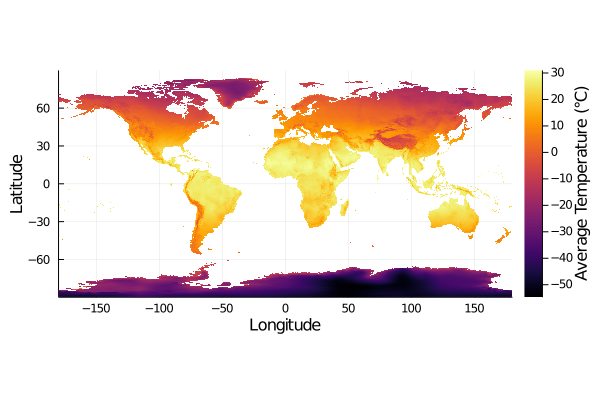
\includegraphics{figures/joss/paper_temp_1.png}
\caption{Map of the average annual temperature data from WorldClim 2.1,
accessed as a layer through SimpleSDMLayers.jl\label{fig:temp}}
\end{figure}

\hypertarget{feature-overview}{%
\section{Feature overview}\label{feature-overview}}

\mintinline[]{text}{SimpleSDMLayers.jl} implements the following
features:

\begin{itemize}
\tightlist
\item
  \textbf{Overloads for common functions}: The
  \mintinline[]{text}{SimpleSDMLayer} types are implemented along with
  overloads for many common functions and operations, such as
  subsetting, changing values, copying, and iterating. Therefore, the
  layers and the raster values stored in the \mintinline[]{text}{grid}
  field can be manipulated as easily as any \mintinline[]{text}{Array},
  without losing their spatial aspect.
\item
  \textbf{Statistical operations on layer values}: Common operations can
  be performed directly on the layer values without worrying about the
  underlying structure (for example, sum, minimum, maximum, mean,
  median).
\item
  \textbf{Statistical operations on multiple layers}: Operations can
  also be performed between layers to produce a new layer, just as
  \mintinline[]{text}{Arrays}, as long as they share the same
  coordinates. For instance, two layers can be added or subtracted, and
  calling \mintinline[]{text}{mean()} will produce a new layer with the
  mean value per pixel.
\item
  \textbf{Spatial operations}: \mintinline[]{text}{SimpleSDMLayers.jl}
  implements spatial operations such as clipping a layer to given
  coordinates, coarsening the resolution by grouping values, and
  performing sliding window operations given a certain radius.
\item
  \textbf{Datasets supported}: The package provides access to climate
  data at different resolutions from WorldClim 2.1 and CHELSA, as well
  as land cover data from EarthEnv. Custom raster data can be loaded as
  well.
\item
  \textbf{Plotting recipes}: Default recipes are implemented for the
  \mintinline[]{text}{SimpleSDMLayer} types, allowing to directly map
  them, view the grid data as histograms and density plots, or compare
  layers as 2-dimensional histograms.
\item
  \textbf{Integration with GBIF.jl (and DataFrames.jl)}:
  \mintinline[]{text}{SimpleSDMLayer.jl} is well integrated with
  \mintinline[]{text}{GBIF.jl}, allowing to clip layers based on the
  occurrence data, as well as to map occurrences by displaying them over
  the layers. Both packages also offer an integration with
  \mintinline[]{text}{DataFrames.jl} to easily convert environmental and
  occurrence data to a table format.
\end{itemize}

\hypertarget{examples}{%
\section{Examples}\label{examples}}

\hypertarget{spatial-operations}{%
\subsubsection{Spatial operations}\label{spatial-operations}}

To illustrate a few of the spatial operations supported by
\mintinline[]{text}{SimpleSDMLayers.jl}, the following code reuses the
previous \mintinline[]{text}{temperature} layer, and shows how it is
possible to : 1) clip the layer to a region of interest (Europe for
instance); 2) coarsen the resolution by averaging groups of cells for
large scale analyses; and 3) perform sliding window operations to
aggregate values for each site based on a certain radius. Each of these
operations can be performed in a single command and returns new layers,
which can then be plotted as shown previously.

\begin{minted}[]{julia}
using Statistics
# Clip to Europe
temperature_europe = temperature[left = -11.2, right = 30.6, bottom = 29.1, top = 71.0]
# Coarsen resolution
temperature_coarse = coarsen(temperature_europe, Statistics.mean, (4, 4))
# Sliding window averaging
temperature_slided = slidingwindow(temperature_europe, Statistics.mean, 100.0)
\end{minted}

\hypertarget{gbif-integration}{%
\subsubsection{GBIF integration}\label{gbif-integration}}

The following example shows how the integration between
\mintinline[]{text}{SimpleSDMLayers.jl} and \mintinline[]{text}{GBIF.jl}
allows to easily map the occurrences of any species in GBIF. The species
represented in this example is the belted kingfisher (\emph{Megaceryle
alcyon}).

\mintinline[]{text}{GBIF.jl} first allows us to retrieve the latest
occurrences from the GBIF database. Note that the element returned here
uses the \mintinline[]{text}{GBIFRecords} format, which contains the
metadata associated to each GBIF occurrence.

\begin{minted}[]{julia}
using GBIF
kingfisher = GBIF.taxon("Megaceryle alcyon", strict=true)
kf_occurrences = occurrences(kingfisher)
# Get at least 200 occurrences
while length(kf_occurrences) < 200
    occurrences!(kf_occurrences)
    @info "$(length(kf_occurrences)) occurrences"
end
kf_occurrences
\end{minted}

\begin{minted}[]{text}
GBIF records: downloaded 200 out of 100000
\end{minted}

\mintinline[]{text}{SimpleSDMLayers.jl} then provides a simple
integration between the occurrence data and the environmental layers.
The layers can be clipped to the spatial extent of the occurrences in a
single call using the \mintinline[]{text}{clip()} function. The
occurrences' coordinates can also be extracted with
\mintinline[]{text}{longitudes()} and \mintinline[]{text}{latitudes()}.
Using these functions, we can easily create a map of the occurrences by
overlaying them on top of the clipped environmental layer
(\autoref{fig:gbif}).

\begin{minted}[]{julia}
# Clip layer to occurrences
temperature_clip = clip(temperature, kf_occurrences)

# Plot occurrences
contour(temperature_clip, fill = true)
scatter!(longitudes(kf_occurrences), latitudes(kf_occurrences))
\end{minted}

\begin{figure}
\centering
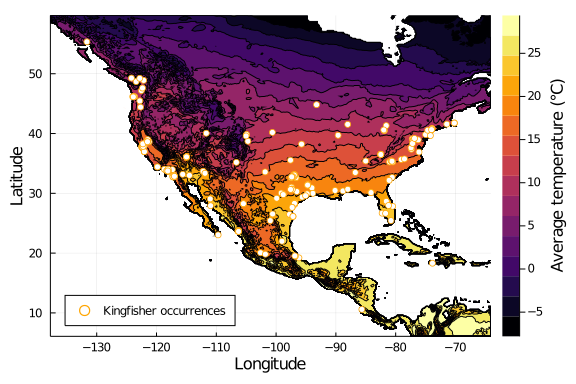
\includegraphics{figures/joss/paper_gbif_1.png}
\caption{Latest belted kingfisher occurrences from the GBIF database
displayed over the temperature data through the integration between
SimpleSDMLayers.jl and GBIF.jl\label{fig:gbif}}
\end{figure}

\hypertarget{acknowledgements}{%
\section{Acknowledgements}\label{acknowledgements}}

We would like to thank all contributors to the \emph{EcoJulia}
organization for their help in developing this series of packages for
ecological research. Funding was provided by Fonds de recherche du
Québec - Nature et technologies (FRQNT) and the Computational
Biodiversity Science and Services (BIOS²) training program.

\end{document}


Exemple de citation~: Consultez le \LaTeX\ companien
de Mittelbach {\it et al\/}\@. \citeyearpar{exemple}.

 % Pour générer la bibliographie à la fin
 % de l'article, utiliser la commande de la
 % classe <dms> \sectionbibliography{<nom du .bib>}.
 % Il y a aussi la possibilité d'utiliser le package
 % <chapterbib>, auquel cas on utilise simplement
 % \bibliography normalement.
 %
 % IMPORTANT : Dans tous les cas, il faut faire
 %    pdflatex these
 %    bibtex chapitre1
 %    bibtex chapitre2
 %    .
 %    .
 %    .
 %    bibtex chapitreN
 %    pdflatex these
 %    pdflatex these
 %
 % où <these> est le nom du .tex principal
 % (qui contient le \documentclass).
 % bibtex a besoin du .aux de chapitre1 et
 % non du .tex. Il est parfois nécessaire
 % d'effacer le .aux et de recommencer la
 % compilation du début.
%%\bibliographystyle{plain} % style plain anglais ou
% \bibliographystyle{plain-fr} % style plain francais
% \bibliographystyle{plainnat-fr}
\bibliographystyle{apalike-fr}
%%\bibliographystyle{<style>} % autre
\sectionbibliography{ref.bib} %Donner le nom du .bib

\endinput
%%
%% End of file `article1.tex'.
